\section{Schnittstellen innerhalb der Software} \label{Softwareschnittstellen}

	Die Software besteht aus den drei Hauptelementen: Bedienung und Beobachtung (HMI), Prozessmodell und Anlagenmodell (Abb. \ref{fig:Strukturübersicht}). Um die Schnittstellen zwischen diesen Elementen zu definieren, müssen die Kompetenzen klar definiert werden. Wer ist für was verantwortlich und welche Informationen werden dafür benötigt. 
	
	\textbf{Bedienung und Beobachtung:}
	\vspace{2mm} 
	\\
	Über das HMI wird der Arbeitsplan erstellt und mit den erforderlichen Ablaufparameter versehen. Das System sowie der erstellte Arbeitsplan können über das HMI gestartet, gestoppt und gesteuert werden.
	
	\textbf{Prozessmodell:}
	\vspace{2mm} 
	\\
	Das Prozessmodell koordiniert die Ausführung des Arbeitsplans. Zusammen mit den Ablaufparameter werden die Prozessparameter festgelegt und weitergegeben. Der Arbeitsplan wird in einzelne Skills unterteilt, die wiederum die grundlegenden Funktionen der Anlagenkomponenten ausführen. Die effiziente und standardisierte Definition eines Skills, vereinfacht die Anwendung dieser in den Sequenzen und Arbeitsplänen.
	
	\newpage
	
	\textbf{Anlagenmodell:}
	\vspace{2mm} 
	\\
	Das Anlagenmodell bildet die Funktionalität der Systemkomponenten ab. Es stellt die Funktionen durch Methoden dar, während Zustände und Prozessinformationen über Eigenschaften wiedergegeben werden. Das Anlagenmodell verarbeitet die erhaltenen Prozessparameter und übersetzt diese in Anlagenparameter, mit denen die Komponenten der Anlage betrieben werden. Die vom Anlagenmodell zurückgemeldeten Daten (wie Zustände und Messwerte) werden als Zustandsparameter bezeichnet. 
	\\
	\vspace{-13mm}
	\begin{wrapfigure}{r}{0.35\textwidth}
		\centering
		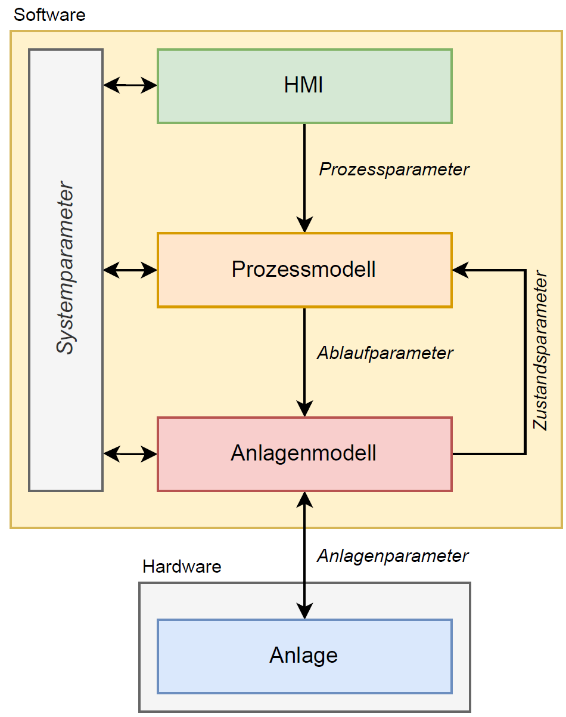
\includegraphics[width=0.3\textwidth]{05_Softwarestruktur/Systemstruktur}
		\captionsetup{justification=centering}
		\caption{Systemstruktur}
		\label{fig:Systemstruktur}
	\end{wrapfigure} \par
	Die drei Hauptelemente müssen voneinander abgegrenzt werden (Abb. \ref{fig:Systemstruktur}). Der modellbasierte Ansatz der Softwarestruktur bietet dabei mehrere Vorteile (siehe EVA-Referenz). Dank klarer Struktur und Übersichtlichkeit lassen sich die Prozesse und Abläufe leicht nachvollziehen. Dies erleichtert die Kommunikation, da durch die einheitliche Verwendung von Begriffen alle dieselbe «Sprache» sprechen. Darüber hinaus können Risiken früher und einfacher erkannt werden.
	\\
	Die Abgrenzung der Hauptelemente geschieht über die Schnittstellen zwischen diesen. Die Schnittstellen werden durch die verschiedenen Parameter definiert. Der Begriff Parameter ist dabei ein Sammelbegriff für alle definierten Variablen, welche zwischen den Elementen ausgetauscht werden.
	
	\textbf{Prozessparameter:}
	\vspace{2mm} 
	\\
	Die Prozessparameter beschreiben den Prozess auf eine möglichst einfache Weise. Es werden nur Informationen weitergegeben, welche nötig sind um den Prozess eindeutig zu definieren. Die Prozessparameter hängen dabei von den Skills und deren Fähigkeiten ab. Die Parameter werden während der Erarbeitung des Prozessmodells definiert.
	
	\textbf{Ablaufparameter:}
	\vspace{2mm} 
	\\
	Ablaufparameter werden durch die Skills definiert und legen relevante Parameter für den Ablauf fest. Die Informationen sind jedoch nicht konkret auf die Komponenten im System ausgelegt. Die Ablaufparameter sind noch anlagenunabhängig und hängen z.B. nicht vom Typ des Roboters ab, welcher im System eingesetzt wird. Die genauen Parameter werden während der Erarbeitung des Prozessmodells definiert.
	
	\textbf{Anlagenparameter:}
	\vspace{2mm} 
	\\
	Die Parameter, welche von den instanziierten Objekten im Anlagemodell vorbereitet werden, dienen als Schnittstelle zur realen Anlage und sind anlagenspezifisch. Die Art dieser Parameter hängt von den eingesetzten Komponenten im System ab. Die genauen Parameter werden während der Erarbeitung des Anlagenmodells definiert.
	
	\textbf{Zustandsparameter:}
	\vspace{2mm} 
	\\
	Die durch die instanziierten Objekte ausgewerteten und verarbeiteten Anlagenparameter werden als Zustandsparameter an das Prozessmodell zurückgegeben. Auf diese Parameter reagiert der Skill wie auch das System. Die genauen Parameter werden während der Erarbeitung des Anlagenmodells definiert.
	
	\textbf{Systemparameter:}
	\vspace{2mm} 
	\\
	Systemparameter sind systemübergreifende Parameter, welche zur Bedienung des gesamten Systems verwendet werden oder dessen Zustand darstellen. 